\documentclass[12pt]{article}

% PACKAGE IMPORTS
\usepackage{fancyhdr}
\usepackage[utf8]{inputenc}
\usepackage[T1]{fontenc}
\usepackage[english]{babel}
\usepackage{graphicx}
\usepackage{blindtext}
\usepackage{titlesec}
\usepackage{csquotes}
\usepackage{enumitem}
\usepackage{amsfonts}
\usepackage[font=small,skip=0pt]{caption}
\usepackage{subcaption}
\usepackage{hyperref}
\hypersetup{hidelinks} % no red boxes around links
\usepackage{float}
\usepackage{xcolor}
\usepackage{amsmath,esint}
\usepackage{booktabs}
\usepackage{adjustbox}
\usepackage{calc}
\usepackage{colortbl}
\usepackage{array}
\usepackage{etoolbox}
\usepackage{wrapfig}
\usepackage{ragged2e}
\usepackage{textcomp, gensymb}
\usepackage{pdflscape}
\usepackage{pdfpages}
\usepackage{tikz} % Used for positioning text on title
\usepackage{geometry} % Used for adjusting the margins
\usepackage{lastpage} % Used for adding a page count to the footer
\usepackage[scaled]{helvet} % Helvetica font
\usepackage{soul} % Used for custom letter spacing on title page
\usepackage{eso-pic}
\usepackage[useregional]{datetime2}
\usepackage{longtable}
% added for this report
\usepackage{amssymb}
\usepackage{siunitx}
\sisetup{detect-all}
\usepackage{tabularx}

% SCREENSHOT PATH
\graphicspath{{pictures/template/}{figures/}}

\PassOptionsToPackage{x11names}{xcolor} % Used for adding colors

% FONT SETTINGS
\renewcommand\familydefault{\sfdefault} % Set default font to sans-serif

% DEFINE COLORS
\definecolor{ertred}{RGB}{226,12,24} % Rocket team's red for header and footer lines
\definecolor{issuccess}{RGB}{0,115,10}
\definecolor{isdanger}{RGB}{200,10,10}

% NUMBERS QUOTED IN THE TEXT (generated by studies/total_length.py)
% generated by studies/total_length.py -- do not edit
\newcommand{\TLInVKC}{\SI{155}{mm}}
\newcommand{\TLInVKL}{\SI{495}{mm}}
\newcommand{\TLInVKLD}{2.75}
\newcommand{\TLInVKAPO}{\SI{8647}{m}}
\newcommand{\TLInVKD}{\SI{-353}{m}}
\newcommand{\TLInVKP}{\SI{-0}{mm}}
\newcommand{\TLInVKLIN}{\SI{155}{mm}}
\newcommand{\TLInVKINC}{\SI{155}{mm}}
\newcommand{\TLInVKCAN}{\SI{209}{mm}}
\newcommand{\TLInVKMASS}{\SI{327}{g}}
\newcommand{\TLInVKFDMASS}{\SI{422}{g}}
\newcommand{\TLInVKLEFT}{\SI{978}{g}}
\newcommand{\TLInVKDSM}{$-$0.047}
\newcommand{\TLInVKMNOSE}{\SI{5.74}{kg}}
\newcommand{\TLInVKFMAX}{\SI{810}{N}}
\newcommand{\TLInVKFULT}{\SI{1620}{N}}
\newcommand{\TLInVKFLIFT}{\SI{344}{N}}
\newcommand{\TLInVKFDRAG}{\SI{403}{N}}
\newcommand{\TLInVKFDRAGPCT}{\SI{50}{\percent}}
\newcommand{\TLInVKREQSEVEN}{\SI{2.25}{kN}}
\newcommand{\TLInVKBEND}{\SI{46}{N.m}}
\newcommand{\TLInVKALPHA}{\ang{2.2}}
\newcommand{\TLInVKQMAX}{\SI{129}{kPa}}
\newcommand{\TLInVKMQ}{1.54}
\newcommand{\TLInVKARM}{\SI{402}{mm}}
\newcommand{\TLInVKXCP}{\SI{244}{mm}}
\newcommand{\TLInVKMMAX}{1.45}
\newcommand{\TLInVKMMAXENV}{1.54}
\newcommand{\TLInVKTIP}{\SI{81}{\celsius}}
\newcommand{\TLInVKBOND}{\SI{94}{\celsius}}
\newcommand{\TLInVKBONDNOM}{\SI{69}{\celsius}}
\newcommand{\TLInVKSHELL}{\SI{102}{\celsius}}
\newcommand{\TLInVKSHELLNOM}{\SI{76}{\celsius}}
\newcommand{\TLInVKTZERO}{\SI{425}{K}}
\newcommand{\TLInVKTZEROC}{\SI{152}{\celsius}}
\newcommand{\TLInVKFILE}{\texttt{nose\_vonkarman\_L495\_c155\_rn4.5mm}}
\newcommand{\TLInVKPHYS}{\SI{491.9}{mm}}
\newcommand{\TLInVKTOTPHYS}{\SI{646.9}{mm}}
\newcommand{\TLInVKTRUNC}{\SI{3.1}{mm}}
\newcommand{\TLInVKXGRV}{\SI{337}{mm}}
\newcommand{\TLInLVHC}{\SI{89}{mm}}
\newcommand{\TLInLVHL}{\SI{561}{mm}}
\newcommand{\TLInLVHLD}{3.12}
\newcommand{\TLInLVHAPO}{\SI{8703}{m}}
\newcommand{\TLInLVHD}{\SI{-297}{m}}
\newcommand{\TLInLVHP}{\SI{-1}{mm}}
\newcommand{\TLInLVHLIN}{\SI{222}{mm}}
\newcommand{\TLInLVHINC}{\SI{88}{mm}}
\newcommand{\TLInLVHCAN}{\SI{220}{mm}}
\newcommand{\TLInLVHMASS}{\SI{329}{g}}
\newcommand{\TLInLVHFDMASS}{\SI{424}{g}}
\newcommand{\TLInLVHLEFT}{\SI{976}{g}}
\newcommand{\TLInLVHDSM}{$-$0.049}
\newcommand{\TLInLVHMNOSE}{\SI{5.74}{kg}}
\newcommand{\TLInLVHFMAX}{\SI{796}{N}}
\newcommand{\TLInLVHFULT}{\SI{1593}{N}}
\newcommand{\TLInLVHFLIFT}{\SI{344}{N}}
\newcommand{\TLInLVHFDRAG}{\SI{388}{N}}
\newcommand{\TLInLVHFDRAGPCT}{\SI{49}{\percent}}
\newcommand{\TLInLVHREQSEVEN}{\SI{2.25}{kN}}
\newcommand{\TLInLVHBEND}{\SI{47}{N.m}}
\newcommand{\TLInLVHALPHA}{\ang{2.1}}
\newcommand{\TLInLVHQMAX}{\SI{130}{kPa}}
\newcommand{\TLInLVHMQ}{1.55}
\newcommand{\TLInLVHARM}{\SI{405}{mm}}
\newcommand{\TLInLVHXCP}{\SI{243}{mm}}
\newcommand{\TLInLVHMMAX}{1.46}
\newcommand{\TLInLVHMMAXENV}{1.55}
\newcommand{\TLInLVHTIP}{\SI{84}{\celsius}}
\newcommand{\TLInLVHBOND}{\SI{93}{\celsius}}
\newcommand{\TLInLVHBONDNOM}{\SI{69}{\celsius}}
\newcommand{\TLInLVHSHELL}{\SI{102}{\celsius}}
\newcommand{\TLInLVHSHELLNOM}{\SI{76}{\celsius}}
\newcommand{\TLInLVHTZERO}{\SI{426}{K}}
\newcommand{\TLInLVHTZEROC}{\SI{153}{\celsius}}
\newcommand{\TLInLVHFILE}{\texttt{nose\_lvhaack\_L561\_c89\_rn4.5mm}}
\newcommand{\TLInLVHPHYS}{\SI{558.7}{mm}}
\newcommand{\TLInLVHTOTPHYS}{\SI{647.7}{mm}}
\newcommand{\TLInLVHTRUNC}{\SI{2.3}{mm}}
\newcommand{\TLInLVHXGRV}{\SI{337}{mm}}
\newcommand{\TLInPHC}{\SI{186}{mm}}
\newcommand{\TLInPHL}{\SI{464}{mm}}
\newcommand{\TLInPHLD}{2.58}
\newcommand{\TLInPHAPO}{\SI{8621}{m}}
\newcommand{\TLInPHD}{\SI{-379}{m}}
\newcommand{\TLInPHP}{\SI{-0}{mm}}
\newcommand{\TLInPHLIN}{\SI{124}{mm}}
\newcommand{\TLInPHINC}{\SI{186}{mm}}
\newcommand{\TLInPHCAN}{\SI{242}{mm}}
\newcommand{\TLInPHMASS}{\SI{337}{g}}
\newcommand{\TLInPHFDMASS}{\SI{432}{g}}
\newcommand{\TLInPHLEFT}{\SI{968}{g}}
\newcommand{\TLInPHDSM}{$-$0.060}
\newcommand{\TLInPHMNOSE}{\SI{5.74}{kg}}
\newcommand{\TLInPHFMAX}{\SI{834}{N}}
\newcommand{\TLInPHFULT}{\SI{1669}{N}}
\newcommand{\TLInPHFLIFT}{\SI{344}{N}}
\newcommand{\TLInPHFDRAG}{\SI{431}{N}}
\newcommand{\TLInPHFDRAGPCT}{\SI{52}{\percent}}
\newcommand{\TLInPHREQSEVEN}{\SI{2.25}{kN}}
\newcommand{\TLInPHBEND}{\SI{48}{N.m}}
\newcommand{\TLInPHALPHA}{\ang{2.1}}
\newcommand{\TLInPHQMAX}{\SI{129}{kPa}}
\newcommand{\TLInPHMQ}{1.54}
\newcommand{\TLInPHARM}{\SI{418}{mm}}
\newcommand{\TLInPHXCP}{\SI{232}{mm}}
\newcommand{\TLInPHMMAX}{1.45}
\newcommand{\TLInPHMMAXENV}{1.54}
\newcommand{\TLInPHTIP}{\SI{91}{\celsius}}
\newcommand{\TLInPHBOND}{\SI{94}{\celsius}}
\newcommand{\TLInPHBONDNOM}{\SI{69}{\celsius}}
\newcommand{\TLInPHSHELL}{\SI{101}{\celsius}}
\newcommand{\TLInPHSHELLNOM}{\SI{75}{\celsius}}
\newcommand{\TLInPHTZERO}{\SI{425}{K}}
\newcommand{\TLInPHTZEROC}{\SI{152}{\celsius}}
\newcommand{\TLInPHFILE}{\texttt{nose\_power050\_L464\_c186\_rn4.5mm}}
\newcommand{\TLInPHPHYS}{\SI{464.0}{mm}}
\newcommand{\TLInPHTOTPHYS}{\SI{650.0}{mm}}
\newcommand{\TLInPHTRUNC}{\SI{0.0}{mm}}
\newcommand{\TLInPHXGRV}{\SI{340}{mm}}
\newcommand{\TLOutVKC}{\SI{20}{mm}}
\newcommand{\TLOutVKL}{\SI{630}{mm}}
\newcommand{\TLOutVKLD}{3.50}
\newcommand{\TLOutVKAPO}{\SI{8905}{m}}
\newcommand{\TLOutVKD}{\SI{-95}{m}}
\newcommand{\TLOutVKP}{\SI{93}{mm}}
\newcommand{\TLOutVKLIN}{\SI{197}{mm}}
\newcommand{\TLOutVKINC}{\SI{20}{mm}}
\newcommand{\TLOutVKCAN}{\SI{496}{mm}}
\newcommand{\TLOutVKMASS}{\SI{300}{g}}
\newcommand{\TLOutVKFDMASS}{\SI{395}{g}}
\newcommand{\TLOutVKLEFT}{\SI{1005}{g}}
\newcommand{\TLOutVKDSM}{$+$0.018}
\newcommand{\TLOutVKMNOSE}{\SI{1.75}{kg}}
\newcommand{\TLOutVKFMAX}{\SI{418}{N}}
\newcommand{\TLOutVKFULT}{\SI{836}{N}}
\newcommand{\TLOutVKFLIFT}{\SI{105}{N}}
\newcommand{\TLOutVKFDRAG}{\SI{290}{N}}
\newcommand{\TLOutVKFDRAGPCT}{\SI{69}{\percent}}
\newcommand{\TLOutVKREQSEVEN}{\SI{0.69}{kN}}
\newcommand{\TLOutVKBEND}{\SI{39}{N.m}}
\newcommand{\TLOutVKALPHA}{\ang{2.5}}
\newcommand{\TLOutVKQMAX}{\SI{132}{kPa}}
\newcommand{\TLOutVKMQ}{1.56}
\newcommand{\TLOutVKARM}{\SI{335}{mm}}
\newcommand{\TLOutVKXCP}{\SI{310}{mm}}
\newcommand{\TLOutVKMMAX}{1.47}
\newcommand{\TLOutVKMMAXENV}{1.56}
\newcommand{\TLOutVKTIP}{\SI{77}{\celsius}}
\newcommand{\TLOutVKBOND}{\SI{95}{\celsius}}
\newcommand{\TLOutVKBONDNOM}{\SI{69}{\celsius}}
\newcommand{\TLOutVKSHELL}{\SI{104}{\celsius}}
\newcommand{\TLOutVKSHELLNOM}{\SI{77}{\celsius}}
\newcommand{\TLOutVKTZERO}{\SI{428}{K}}
\newcommand{\TLOutVKTZEROC}{\SI{155}{\celsius}}
\newcommand{\TLOutVKFILE}{\texttt{nose\_vonkarman\_L630\_c20\_rn4.5mm}}
\newcommand{\TLOutVKPHYS}{\SI{625.4}{mm}}
\newcommand{\TLOutVKTOTPHYS}{\SI{645.4}{mm}}
\newcommand{\TLOutVKTRUNC}{\SI{4.6}{mm}}
\newcommand{\TLOutVKXGRV}{\SI{428}{mm}}
\newcommand{\TLOutLVHC}{\SI{20}{mm}}
\newcommand{\TLOutLVHL}{\SI{630}{mm}}
\newcommand{\TLOutLVHLD}{3.50}
\newcommand{\TLOutLVHAPO}{\SI{8836}{m}}
\newcommand{\TLOutLVHD}{\SI{-164}{m}}
\newcommand{\TLOutLVHP}{\SI{41}{mm}}
\newcommand{\TLOutLVHLIN}{\SI{249}{mm}}
\newcommand{\TLOutLVHINC}{\SI{20}{mm}}
\newcommand{\TLOutLVHCAN}{\SI{527}{mm}}
\newcommand{\TLOutLVHMASS}{\SI{317}{g}}
\newcommand{\TLOutLVHFDMASS}{\SI{412}{g}}
\newcommand{\TLOutLVHLEFT}{\SI{988}{g}}
\newcommand{\TLOutLVHDSM}{$-$0.020}
\newcommand{\TLOutLVHMNOSE}{\SI{1.75}{kg}}
\newcommand{\TLOutLVHFMAX}{\SI{459}{N}}
\newcommand{\TLOutLVHFULT}{\SI{917}{N}}
\newcommand{\TLOutLVHFLIFT}{\SI{105}{N}}
\newcommand{\TLOutLVHFDRAG}{\SI{332}{N}}
\newcommand{\TLOutLVHFDRAGPCT}{\SI{72}{\percent}}
\newcommand{\TLOutLVHREQSEVEN}{\SI{0.69}{kN}}
\newcommand{\TLOutLVHBEND}{\SI{44}{N.m}}
\newcommand{\TLOutLVHALPHA}{\ang{2.3}}
\newcommand{\TLOutLVHQMAX}{\SI{131}{kPa}}
\newcommand{\TLOutLVHMQ}{1.55}
\newcommand{\TLOutLVHARM}{\SI{374}{mm}}
\newcommand{\TLOutLVHXCP}{\SI{273}{mm}}
\newcommand{\TLOutLVHMMAX}{1.46}
\newcommand{\TLOutLVHMMAXENV}{1.55}
\newcommand{\TLOutLVHTIP}{\SI{82}{\celsius}}
\newcommand{\TLOutLVHBOND}{\SI{94}{\celsius}}
\newcommand{\TLOutLVHBONDNOM}{\SI{69}{\celsius}}
\newcommand{\TLOutLVHSHELL}{\SI{103}{\celsius}}
\newcommand{\TLOutLVHSHELLNOM}{\SI{77}{\celsius}}
\newcommand{\TLOutLVHTZERO}{\SI{427}{K}}
\newcommand{\TLOutLVHTZEROC}{\SI{154}{\celsius}}
\newcommand{\TLOutLVHFILE}{\texttt{nose\_lvhaack\_L630\_c20\_rn4.5mm}}
\newcommand{\TLOutLVHPHYS}{\SI{627.1}{mm}}
\newcommand{\TLOutLVHTOTPHYS}{\SI{647.1}{mm}}
\newcommand{\TLOutLVHTRUNC}{\SI{2.9}{mm}}
\newcommand{\TLOutLVHXGRV}{\SI{378}{mm}}
\newcommand{\TLOutPHC}{\SI{20}{mm}}
\newcommand{\TLOutPHL}{\SI{630}{mm}}
\newcommand{\TLOutPHLD}{3.50}
\newcommand{\TLOutPHAPO}{\SI{8911}{m}}
\newcommand{\TLOutPHD}{\SI{-89}{m}}
\newcommand{\TLOutPHP}{\SI{121}{mm}}
\newcommand{\TLOutPHLIN}{\SI{169}{mm}}
\newcommand{\TLOutPHINC}{\SI{20}{mm}}
\newcommand{\TLOutPHCAN}{\SI{530}{mm}}
\newcommand{\TLOutPHMASS}{\SI{306}{g}}
\newcommand{\TLOutPHFDMASS}{\SI{401}{g}}
\newcommand{\TLOutPHLEFT}{\SI{999}{g}}
\newcommand{\TLOutPHDSM}{$+$0.021}
\newcommand{\TLOutPHMNOSE}{\SI{1.75}{kg}}
\newcommand{\TLOutPHFMAX}{\SI{427}{N}}
\newcommand{\TLOutPHFULT}{\SI{854}{N}}
\newcommand{\TLOutPHFLIFT}{\SI{105}{N}}
\newcommand{\TLOutPHFDRAG}{\SI{299}{N}}
\newcommand{\TLOutPHFDRAGPCT}{\SI{70}{\percent}}
\newcommand{\TLOutPHREQSEVEN}{\SI{0.69}{kN}}
\newcommand{\TLOutPHBEND}{\SI{39}{N.m}}
\newcommand{\TLOutPHALPHA}{\ang{2.5}}
\newcommand{\TLOutPHQMAX}{\SI{132}{kPa}}
\newcommand{\TLOutPHMQ}{1.56}
\newcommand{\TLOutPHARM}{\SI{335}{mm}}
\newcommand{\TLOutPHXCP}{\SI{315}{mm}}
\newcommand{\TLOutPHMMAX}{1.47}
\newcommand{\TLOutPHMMAXENV}{1.56}
\newcommand{\TLOutPHTIP}{\SI{89}{\celsius}}
\newcommand{\TLOutPHBOND}{\SI{95}{\celsius}}
\newcommand{\TLOutPHBONDNOM}{\SI{69}{\celsius}}
\newcommand{\TLOutPHSHELL}{\SI{104}{\celsius}}
\newcommand{\TLOutPHSHELLNOM}{\SI{77}{\celsius}}
\newcommand{\TLOutPHTZERO}{\SI{428}{K}}
\newcommand{\TLOutPHTZEROC}{\SI{155}{\celsius}}
\newcommand{\TLOutPHFILE}{\texttt{nose\_power050\_L630\_c20\_rn4.5mm}}
\newcommand{\TLOutPHPHYS}{\SI{630.0}{mm}}
\newcommand{\TLOutPHTOTPHYS}{\SI{650.0}{mm}}
\newcommand{\TLOutPHTRUNC}{\SI{-0.0}{mm}}
\newcommand{\TLOutPHXGRV}{\SI{461}{mm}}
\newcommand{\TLGAPVK}{\SI{56}{m}}
\newcommand{\TLGAPPH}{\SI{83}{m}}
\newcommand{\TLEQGAP}{\SI{69}{m}}
\newcommand{\TLEQGAPPH}{\SI{7}{m}}
\newcommand{\TLAB}{\SI{201}{m}}
\newcommand{\TLDZDM}{\SI{143}{m/kg}}
\newcommand{\TLABKG}{\SI{1.4}{kg}}
\newcommand{\TLInKG}{\SI{2.1}{kg}}
\newcommand{\TLOutKG}{\SI{0.7}{kg}}
\newcommand{\TLGRVLEN}{\SI{300}{mm}}
\newcommand{\TLCANMASS}{\SI{0.35}{kg}}
\newcommand{\TLCMIN}{\SI{20}{mm}}
\newcommand{\TLREST}{\SI{4.68}{m}}
\newcommand{\TLLVSIX}{\SI{5.33}{m}}
\newcommand{\TLLVNOSE}{\SI{720}{mm}}
\newcommand{\TLGRVSM}{0.04}
\newcommand{\TLInSLOPE}{\SI{2.7}{m/mm}}
\newcommand{\TLInSEVEN}{\SI{8837}{m}}
\newcommand{\TLInSEVENTWENTY}{\SI{8874}{m}}
\newcommand{\TLInSEVENTWENTYG}{\SI{+171}{m}}
\newcommand{\TLInSHARE}{\SI{58}{\percent}}
\newcommand{\TLInSEVENFIFTY}{\SI{8923}{m}}
\newcommand{\TLInNINE}{\SI{830}{mm}}
\newcommand{\TLInNINELV}{\SI{5.51}{m}}
\newcommand{\TLInNINESHAPE}{Von K\'arm\'an}
\newcommand{\TLOutSLOPE}{\SI{1.1}{m/mm}}
\newcommand{\TLOutSEVEN}{\SI{8958}{m}}
\newcommand{\TLOutSEVENTWENTY}{\SI{8976}{m}}
\newcommand{\TLOutSEVENTWENTYG}{\SI{+71}{m}}
\newcommand{\TLOutSHARE}{\SI{75}{\percent}}
\newcommand{\TLOutSEVENFIFTY}{\SI{9000}{m}}
\newcommand{\TLOutNINE}{\SI{750}{mm}}
\newcommand{\TLOutNINELV}{\SI{5.43}{m}}
\newcommand{\TLOutNINESHAPE}{Von K\'arm\'an}
\newcommand{\TLSENSVKC}{\SI{214}{mm}}
\newcommand{\TLSENSVKD}{\SI{-520}{m}}
\newcommand{\TLSENSLVHC}{\SI{156}{mm}}
\newcommand{\TLSENSLVHD}{\SI{-431}{m}}
\newcommand{\TLSENSPHC}{\SI{241}{mm}}
\newcommand{\TLSENSPHD}{\SI{-561}{m}}


% MARGINS
\geometry{
a4paper,
inner=20mm,
outer=20mm,
top=26mm,
bottom=30mm,
footskip=10mm,
headsep=13mm
}

% TITLE - INTER LETTER SPACING
\sodef\an{}{.1em}{0.1em}{0.1em} % Adjust letter spacing in the title

% FRONT PAGE BACKGROUND IMAGE
\newcommand\BackgroundPic{
\put(0,0){
\parbox[b][\paperheight]{\paperwidth}{
\vfill
\centering

\includegraphics[width=\paperwidth,height=\paperheight]{pictures/template/c_title-page.png} % Background title page image
\vfill
}
}
}

\begin{document}

\AddToShipoutPicture*{\BackgroundPic}
\ClearShipoutPicture

% HEADER AND FOOTER

% HEADER AND FOOTER POSITIONING
\let\oldheadrule\headrule
\renewcommand{\headrule}{\color{ertred}\oldheadrule} % Add color to headrule
\renewcommand{\headrulewidth}{1.5pt}
\renewcommand{\footrule}{\hbox to\headwidth{\color{ertred}\leaders\hrule height \footrulewidth\hfill}}
\renewcommand{\footrulewidth}{1.5pt}
\setlength\headheight{48pt}

% HEADER OPTIONS
\pagestyle{fancy}
\fancyhead[C]{\rule[-2ex]{0pt}{2ex} \bf{ \fontsize{12}{5} \selectfont 2026\_C\_FD\_REPORT-2\_NOSE\_CONE}} % Header document name
\lhead{}
\lhead{
\includegraphics[height=1.5cm]{pictures/template/ert_logo_small}\vspace{-4mm}} % ERT Logo
\rhead{
\includegraphics[height=1.5cm]{pictures/template/c_patch.png}\vspace{-4mm}} % Project Logo

% FOOTER OPTIONS
\cfoot{}
\fancyfoot[R]{\bf{\thepage/\pageref{LastPage}}}
\fancyfoot[L]{\rule[-2ex]{0pt}{2ex}\bf{EPFL ROCKET TEAM}} % Footer Name

% TITLE PAGE
\begin{titlepage}
\vspace*{-2.40cm} % Push title to the top of the page
\noindent
\hspace*{-1.2cm}
\parbox{\linewidth}{%
\bfseries\fontsize{34}{38}\selectfont
REPORT 2 -\\
NOSE CONE ANALYSIS\\ FOR 650MM LENGTH\\
}
\newline
\hspace*{-1.2cm}
\parbox{\linewidth}{%
\bfseries\fontsize{14}{18}\selectfont
Fabio Feig - 315169 \\ % Names and scipers
}

% ADDITIONAL TITLE PAGE DETAILS
\begin{tikzpicture}[remember picture,overlay]
\node[anchor=south east,inner sep=39mm] at (current page.south east) {
\parbox[b][-2.37cm][t]{15cm}{
\raggedleft
\fontsize{12}{12} \selectfont \normalfont \textbf{Weisshorn -- Nose Cone at 650 mm, with and without the 3U}
}
};
\end{tikzpicture}

\begin{tikzpicture}[remember picture,overlay]
\node[anchor=south east,inner sep=39mm] at (current page.south east) {
\parbox[b][-0.8cm][t]{15cm}{
\raggedleft
\fontsize{12}{12} \selectfont \normalfont Date: \today % Date
}
};
\end{tikzpicture}

\begin{tikzpicture}[remember picture,overlay]
\node[anchor=south east,inner sep=39mm] at (current page.south east) {
\parbox[b][-1.6cm][t]{15cm}{
\raggedleft
\fontsize{12}{12} \selectfont \normalfont Doc ID: 2026\_C\_FD\_REPORT-2\_NOSE\_CONE
}
};
\end{tikzpicture}

\end{titlepage}

% TABLE OF CONTENTS
\pagenumbering{roman} % front matter numbered i, ii so the report body starts at 1
\setcounter{tocdepth}{2} % sections and subsections only
{\small\tableofcontents}
\newpage

% PAGE NUMBERING
\pagenumbering{arabic}
\setcounter{page}{1}

% MAIN CONTENT
\section*{Summary}
\addcontentsline{toc}{section}{Summary}

\noindent\fbox{\parbox{\dimexpr\textwidth-2\fboxsep-2\fboxrule}{%
\textbf{Weisshorn nose cone at \SI{650}{mm} (curved part + coupler cylinder): two studies}\\[3pt]
\begin{tabular}{@{}>{\raggedright}p{2.9cm}>{\raggedright}p{6.15cm}>{\raggedright\arraybackslash}p{6.15cm}@{}}
 & \textbf{A: 3U in the nose} (as required) & \textbf{B: 3U not in the nose} \\
Profile & LV-Haack (Haack $C=\tfrac13$) & Von K\'arm\'an (Haack $C=0$) \\
Length & \TLInLVHL{} curved + \TLInLVHC{} coupler & \TLOutVKL{} curved + \TLOutVKC{} coupler \\
Apogee (model) & \TLInLVHAPO{} (\TLInLVHD{} vs.\ \SI{9}{km}) & \TLOutVKAPO{} (\TLOutVKD) \\
\SI{9}{km} needs & \TLInNINE{} total (LV \TLInNINELV) & \TLOutNINE{} total (LV \TLOutNINELV) \\
Both & \multicolumn{2}{p{12.3cm}}{\raggedright \SI{180}{mm} diameter; spherical tip $r_n=\SI{4.5}{mm}$;
CanSat in the nose} \\
\end{tabular}}}

\vspace{6pt}
\noindent The structure requirements cap the nose at \SI{650}{mm}, curved part and cylindrical part
(coupler) together, and put the 3U payload ($100\times100\times\SI{300}{mm}$, the guided recovery
vehicle) in the nose; SE specified that if the 3U does not fit, the nose is extended with a
cylindrical part. This report redoes the design of report~1 (\SI{810}{mm} Von K\'arm\'an) under these
limits for the three best profiles of report~1, with the 3U in the nose (study~A) and without it
(study~B), and gives the apogee of a longer nose for the interface meeting. It covers the FD scope
(profile, lengths, drag, apogee, stability); joint loads, heating and the mass budget are left to ST.

\begin{itemize}[leftmargin=*,itemsep=2pt]
\item \textbf{A: the 3U decides the profile.} The 3U needs a \SI{77}{mm} radius, which a slender nose
reaches only near its base, so the cylinder has to grow, and every millimetre of it is taken from the
curved part. LV-Haack is the fullest near the base and needs the shortest cylinder
(\TLInLVHC): it flies \TLGAPVK{} higher than Von K\'arm\'an (\TLInVKC{} cylinder) and
\TLGAPPH{} higher than power~$\tfrac12$ (\TLInPHC).
\item \textbf{B: the shortest cylinder and the lowest drag.} Without the 3U the cylinder is only the
\TLCMIN{} coupler overlap and Von K\'arm\'an is the lowest-drag profile (power~$\tfrac12$ is within
\TLEQGAPPH, but meets the cylinder at an angle). With this nose the 3U would reach \TLOutVKP{} past
the joint, more than the \SI{50}{mm} free in the RE tube, so it has to go elsewhere in the vehicle.
\item \textbf{For the interface meeting.} Taking the 3U out of the nose is worth \TLAB{} at
\SI{650}{mm}, as much as \TLABKG{} of dry mass (\TLDZDM). A longer nose is worth \TLInSLOPE{} in A
and \TLOutSLOPE{} in B near \SI{650}{mm}. With the rest of the LVO unchanged the
\SI{5.4}{m} LV cap (SE\_REQ\_04) is reached at a \TLLVNOSE{} nose, which gives \TLInSEVENTWENTYG{}
in A and \TLOutSEVENTWENTYG{} in B, \TLInSHARE{} and \TLOutSHARE{} of the shortfall to \SI{9}{km}.
Neither study reaches \SI{9}{km} within the cap (Table~\ref{tab:length}), so neither gain is
negligible.
\item \textbf{New CFD and CAD.} 24 Euler runs at $L/D = 2.5$ and 3.5 confirm the report-1
interpolation (within 0.8\,\%) and correct the extrapolation below $L/D = 3$ (6--10\,\% too much
wave drag). STEP, STL and profile CSV of the six design points (three profiles, two studies) are in
\texttt{CFD/geometry\_650/} for the Fluent runs.
\end{itemize}

\section{Requirements and Inputs}
\label{sec:inputs}

Report~1 (2026\_C\_FD\_REPORT-1\_NOSE\_CONE) chose the profile for a nose of free length and
recommended a Von K\'arm\'an nose of \SI{810}{mm}. The structure (ST) requirements of Weisshorn now
cap the nose at \SI{650}{mm} in total, and systems engineering (SE) specified that this length is the
curved part plus the cylindrical part (the coupler), and that the nose is extended with a
cylindrical part if the 3U payload does not fit in the curved shape. Table~\ref{tab:req} lists the
requirements that drive the nose; everything else (vehicle, engine, trajectory model, Euler solver)
is unchanged from report~1.

\begin{table}[H]
\centering
\caption{Requirements that drive the nose (sheet 2027\_C\_SE\_REQ unless stated).}
\label{tab:req}
\small
\begin{tabular}{@{}>{\raggedright\arraybackslash}p{4.3cm}>{\raggedright\arraybackslash}p{11.2cm}@{}}
\toprule
Requirement & Content \\
\midrule
ST Nosecone/Payload-Bay Req\_03 & Total length $\leq\SI{650}{mm}$: curved part + cylindrical part (coupler), confirmed by SE \\
Req\_13, Req\_01 & Payload bay prepared for both cases: a CanSat at the front of the nose with a volume for the guided recovery in its lower part, or a 3U volume; if the 3U does not fit, the nose is extended with a cylinder (SE) \\
PL\_GRV\_REQ\_02, \_03 & 3U payload (guided recovery vehicle, GRV) $100\times100\times\SI{300}{mm}$, \SIrange{3.0}{3.99}{kg} \\
ST\_REQ\_09 & Integration diameter through couplers $\geq\SI{155}{mm}$ \\
RE\_REQ\_08 & Recovery (RE) assembly $\leq\SI{550}{mm}$ in a \SI{600}{mm} tube: \SI{50}{mm} free \\
SE\_REQ\_01, \_04 & Apogee $\geq\SI{9000}{m}$ AGL; launch vehicle (LV) shorter than \SI{5.4}{m} \\
\bottomrule
\end{tabular}
\end{table}

\paragraph{The coupler.} As on Firehorn, the coupler ring is bonded inside a full-diameter
cylindrical extension of the nose shell, behind the curved part; its aft face is the joint (the
separation plane) to the RE bay. This cylinder is part of the outer skin, so its length $c$ counts in
the \SI{650}{mm} and is taken from the curved part: $L = \SI{650}{mm} - c$. Its shortest length is
set by ST (bond overlap, separation mechanism, fasteners). The study assumes $c\geq\TLCMIN$; a longer
cylinder is simply a payload bay.

\paragraph{The 3U envelope.} The 3U ($100\times\SI{100}{mm}$ section) needs an outer radius
$r\geq\SI{77}{mm}$: \SI{70.7}{mm} half-diagonal, \SI{3}{mm} clearance, \SI{2}{mm} guide rail and
the \SI{1.2}{mm} shell. This is true only near the base of a slender nose. Its length is taken as
\TLGRVLEN{} (PL\_GRV\_REQ\_02) plus \SI{10}{mm} axial clearance; report~1 used the
\SI{340.5}{mm} of a 3U CubeSat, whose effect is given in Section~\ref{sec:sens}. The coupler ring
leaves at least \SI{155}{mm} free, enough for the \SI{151}{mm} the 3U needs, so the 3U can pass
through it. The CanSat (\O\SI{66}{mm}$\times$\SI{115}{mm}) needs $r\geq\SI{39.2}{mm}$ by the same
rule.

\paragraph{The two studies.}
\begin{itemize}[leftmargin=*,itemsep=1pt]
\item \textbf{Study A, 3U in the nose} (the requirements as written): the cylinder is made as long as
needed for nothing of the 3U to reach past the joint, within the \SI{650}{mm}.
\item \textbf{Study B, 3U not in the nose}: the cylinder is the \TLCMIN{} minimum and the 3U goes
elsewhere in the vehicle. The nose keeps the CanSat.
\end{itemize}
For the interface meeting both studies are repeated for allowed total lengths from 600 to
\SI{850}{mm}. An extension of the cylinder beyond \SI{650}{mm} (the other reading of SE's rule) is a
point of these curves.

\paragraph{Unchanged from report 1.} LVO vehicle (\SI{75}{kg} wet, \SI{4.5}{kN} for \SI{9.1}{s},
\SI{180}{mm}), assumed fins, point-mass trajectory from the \SI{12}{m} rail at $84^\circ$, ISA, and
the drag factor $k$ that makes the LVS vehicle (Von K\'arm\'an, \SI{720}{mm}) reach \SI{9000}{m}.
The apogee shortfalls below are therefore relative to what the LVO assumed; the real margin depends
on the LVO's own margin above \SI{9}{km}. The vehicle behind the nose joint (\TLREST) is the same for
every option: with a \SI{650}{mm} nose the LV is \TLLVSIX{} long, and a longer nose lengthens it by
the same amount.

\section{Method}
\label{sec:method}

The chain of report~1 is reused: the Euler wave drag of each nose feeds a drag build-up and a
point-mass ascent trajectory, which gives the apogee. Three things are new: direct Euler runs at the
short lengths the \SI{650}{mm} limit allows, the fixed-total-length geometry, and the 3U fit. The study is run by
\texttt{studies/total\_length.py} with \texttt{configs/weisshorn\_650.yaml} in the
\texttt{weisshorn-nose-cone} repository.

\paragraph{Profiles.} The three best profiles of report~1 are compared. Von K\'arm\'an (Haack
series $C=0$) has the lowest wave drag for a given length. LV-Haack ($C=\tfrac13$) is the Haack
nose of lowest drag for a given length and volume: it is fuller near the base, which is where the
3U sits. The power-$\tfrac12$ nose ($y = R\sqrt{x/L}$) has almost the same drag as
Von K\'arm\'an at short lengths but is the slimmest at the base. All three get the \SI{4.5}{mm}
spherical tip of report~1.

\paragraph{Wave drag.} Report~1 computed these profiles at $L/D = 3$, 4, 4.5 and 5 and interpolated
$C_{D,\rm w}(L/D)^2$, which slender-body theory predicts to be nearly constant, between them. The
\SI{650}{mm} limit gives $L/D = 2.5$--$3.5$, at and below the edge of that data. The same
axisymmetric Euler solver (HLLC, MUSCL, $160\times80$ cells; validated against Taylor--Maccoll to
0.5\,\% and grid-converged to 0.5--1\,\% in report~1) was therefore run directly at $L/D = 2.5$
and 3.5 for the three profiles at $M = 1.6$, 1.4, 1.2 and 1.1, giving 24 new points (study
\texttt{f650}). The transonic rise below $M = 1.1$ is modelled as in report~1.

\paragraph{Fixed total length.} For a coupler of length $c$, the curved part is
$L = \SI{650}{mm} - c$. The vehicle behind the joint is fixed, so the coupler cylinder adds its
wetted area $\pi D c$ to the skin friction and its shell mass ($\SI{0.98}{kg/m^2}$, the Firehorn
as-built areal density) to the vehicle; the curved shell mass and the tip follow report~1.

\paragraph{3U fit.} With the profile $y(x)$ measured from the apex, the 3U fits in the last
$l_{\rm in}$ of the curved part, where $y \geq r_{\rm req} = \SI{77}{mm}$:
\begin{equation}
l_{\rm in} = L - x^{*}, \qquad y(x^{*}) = r_{\rm req}.
\label{eq:lin}
\end{equation}
For all three profiles $y/R$ depends only on $x/L$, so $l_{\rm in} = \kappa L$ with a constant
$\kappa$: 0.31 for Von K\'arm\'an, 0.39 for LV-Haack and 0.27 for power~$\tfrac12$. Placed as far
forward as possible, the 3U of length $l_{\rm 3U}$ (with its clearance) then occupies the coupler
and reaches
\begin{equation}
p = l_{\rm 3U} - l_{\rm in} - c = l_{\rm 3U} - \kappa\,(\SI{650}{mm}) - (1-\kappa)\,c
\label{eq:p}
\end{equation}
past the joint. Every millimetre of coupler pulls the 3U back by only $1-\kappa$ of a millimetre,
because it also shortens the curved part. The design point of a profile is, in study~A, the
shortest coupler ($\geq\TLCMIN$) with $p\leq0$ and, in study~B, the \TLCMIN{} minimum. For the
interface meeting the same rules are applied with the \SI{650}{mm} replaced by an allowed total length
from 600 to \SI{850}{mm}; the vehicle behind the joint is kept, so the LV grows with the nose.

\paragraph{Stability.} As in report~1: the static-margin change uses Barrowman's nose centre of
pressure $x_{cp} = L - V/A_{\rm ref}$ ($V$ the nose volume) and the nose mass, relative to the LVS
nose.

\section{Results}
\label{sec:results}

\subsection{Wave drag at short lengths}

Table~\ref{tab:cfd} gives the new direct Euler values. At $L/D = 3.5$ the report-1 interpolation
between $L/D = 3$ and 4 is within 0.6\,\% at $M = 1.4$ and 0.8\,\% at $M = 1.2$--1.6, so the
numbers quoted from it earlier hold. Below $L/D = 3$ report~1 had no data and held $C_{D,\rm w}(L/D)^2$
constant; the new runs show that this product keeps falling as the nose gets blunter, so the
extrapolation overestimated the wave drag of the shortest noses by 6--10\,\%. All results below use
the new data. The $M = 1.1$ runs, and the $M = 1.2$ runs of LV-Haack and power~$\tfrac12$ at
$L/D=2.5$, stopped at the 6000-iteration limit with a residual uncertainty of 1--2\,\%, as the
$M = 1.1$ runs of report~1.

\begin{table}[H]
\centering
\caption{Direct Euler wave drag $C_{D,\rm w}$ (sharp apex) and the error of the report-1 model
(interpolation at $L/D = 3.5$, extrapolation from $L/D = 3$ at 2.5).}
\label{tab:cfd}
\small
\begin{tabular}{@{}llrrrrr@{}}
\toprule
Profile & $L/D$ & $M=1.1$ & $M=1.2$ & $M=1.4$ & $M=1.6$ & report-1 model at $M=1.4$ \\
\midrule
Von K\'arm\'an & 2.5 & 0.1156 & 0.1212 & 0.1190 & 0.1155 & $+$5.7\,\% \\
Von K\'arm\'an & 3.5 & 0.0680 & 0.0686 & 0.0667 & 0.0648 & $-$0.4\,\% \\
LV-Haack & 2.5 & 0.1147 & 0.1302 & 0.1356 & 0.1347 & $+$7.1\,\% \\
LV-Haack & 3.5 & 0.0714 & 0.0767 & 0.0776 & 0.0766 & $-$0.6\,\% \\
Power $\tfrac12$ & 2.5 & 0.1052 & 0.1100 & 0.1122 & 0.1119 & $+$9.8\,\% \\
Power $\tfrac12$ & 3.5 & 0.0641 & 0.0665 & 0.0677 & 0.0675 & $-$0.5\,\% \\
\bottomrule
\end{tabular}

\end{table}

\subsection{Coupler length at 650 mm}

\begin{figure}[H]
\centering
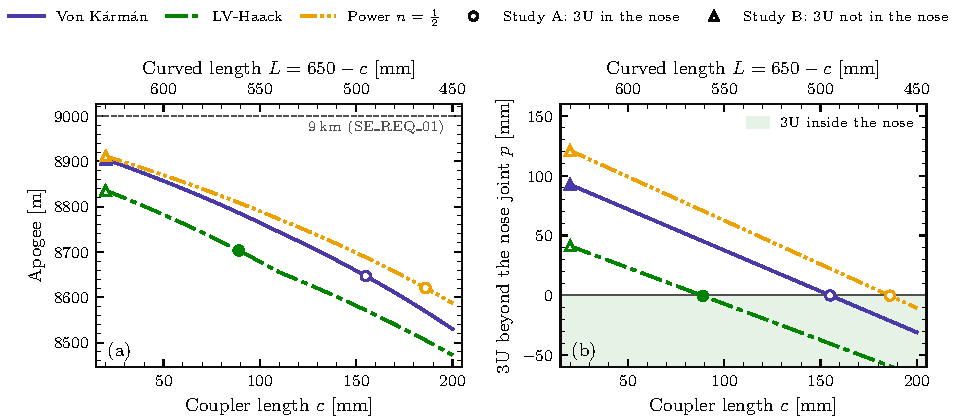
\includegraphics[width=\textwidth]{fig_tl_coupler}
\caption{Total length \SI{650}{mm}. (a) Apogee and (b) length of 3U past the nose joint against
the coupler length $c$. Markers: design point of each profile in study~A (circles) and B
(triangles); filled: the design chosen in each study.}
\label{fig:coupler}
\end{figure}

Figure~\ref{fig:coupler}a shows the cost of the coupler: the apogee falls by \SIrange{1.3}{1.7}{m}
per millimetre of coupler at $c = \TLCMIN$ and by about \SI{2}{m} per millimetre at
$c = \SIrange{100}{150}{mm}$, because the curved part gets shorter and blunter. At
equal length Von K\'arm\'an and power~$\tfrac12$ fly within \TLEQGAPPH{} of each other (the
difference is inside the model uncertainty), and \TLEQGAP{} higher than LV-Haack, as in report~1.

Figure~\ref{fig:coupler}b shows why this ranking does not decide study~A. With the shortest
coupler the 3U reaches \TLOutVKP{} (Von K\'arm\'an) and \TLOutPHP{} (power~$\tfrac12$) past the
joint, and each millimetre of coupler pulls it back by only $1-\kappa$ of a millimetre
(Equation~\ref{eq:p}). LV-Haack has the largest $\kappa$, so its curve starts lowest and reaches
zero first.

\subsection{Design points}

\begin{table}[H]
\centering
\caption{Design point of each profile in each study at \SI{650}{mm}. ``3U in $L$'': length of the
curved part with $r\geq\SI{77}{mm}$; $p$: 3U past the joint (in study~B, where it would reach if it
were in the nose). Bold: best, or within \SI{10}{m} of the best.}
\label{tab:designs}
\small
\begin{tabular}{@{}llrrrrrrr@{}}
\toprule
Study & Profile & $c$ & $L$ & $L/D$ & 3U in $L$ & $p$ & Apogee & vs \SI{9}{km} \\
 & & [mm] & [mm] & & [mm] & [mm] & [m] & [m] \\
\midrule
A: 3U in the nose & Von K\'arm\'an & 155 & 495 & 2.75 & 155 & 0 & 8647 & $-$353 \\
 & \textbf{LV-Haack} & 89 & 561 & 3.12 & 222 & $-$1 & \textbf{8703} & \textbf{$-$297} \\
 & Power $\tfrac12$ & 186 & 464 & 2.58 & 124 & 0 & 8621 & $-$379 \\
\midrule
B: 3U not in the nose & \textbf{Von K\'arm\'an} & 20 & 630 & 3.50 & 197 & 93 & \textbf{8905} & \textbf{$-$95} \\
 & LV-Haack & 20 & 630 & 3.50 & 249 & 41 & 8836 & $-$164 \\
 & \textbf{Power $\tfrac12$} & 20 & 630 & 3.50 & 169 & 121 & \textbf{8911} & \textbf{$-$89} \\
\bottomrule
\end{tabular}

\end{table}

\begin{itemize}[leftmargin=*,itemsep=2pt]
\item \textbf{Study A, 3U in the nose}: LV-Haack, \TLInLVHL{} curved + \TLInLVHC{} coupler,
\TLInLVHD. Von K\'arm\'an needs a \TLInVKC{} coupler, which leaves it only $L/D = \TLInVKLD$, and
loses \TLGAPVK; power~$\tfrac12$ loses \TLGAPPH. If the cylinder may instead be extended beyond
\SI{650}{mm}, keeping a \SI{630}{mm} curved part is not the best use of the extra length: Von
K\'arm\'an 630 + \SI{113}{mm} (\SI{743}{mm}) reaches \SI{8870}{m}, LV-Haack at \SI{740}{mm} in
total \SI{8906}{m} (Section~\ref{sec:length}).
\item \textbf{Study B, 3U not in the nose}: Von K\'arm\'an, \TLOutVKL{} curved + \TLOutVKC{}
coupler, \TLOutVKD; power~$\tfrac12$ (\TLOutPHD) is equal within the model uncertainty, but meets the
cylinder at an angle and is blunt at the tip. The 3U would reach \TLOutVKP{} past the joint, more
than the \SI{50}{mm} free in the RE tube (RE\_REQ\_08), so it has to go elsewhere. Moving it
\SI{100}{mm} aft moves the burn-out centre of gravity aft by about \TLGRVSM~cal, which SE and FD
have to include in the stability budget.
\item \textbf{A against B}: \TLAB{} at \SI{650}{mm}, the apogee of \TLABKG{} of dry mass.
\end{itemize}

\subsection{What a longer nose buys}
\label{sec:length}

\begin{figure}[H]
\centering
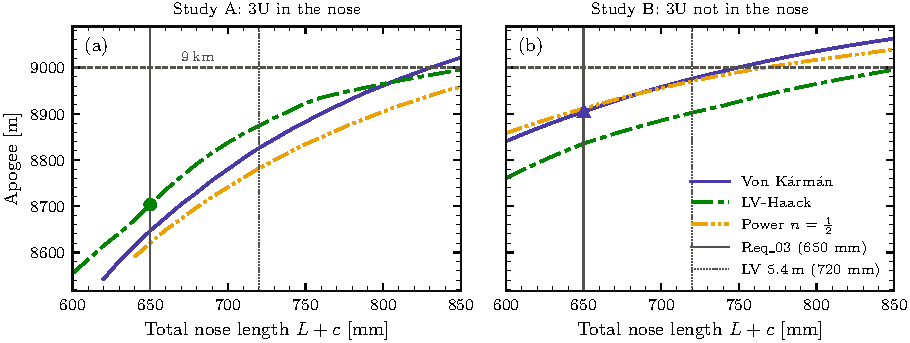
\includegraphics[width=\textwidth]{fig_tl_total}
\caption{Apogee against the allowed total length of the nose, each profile with the coupler of its
study. Solid vertical line: Req\_03; dotted: LV length \SI{5.4}{m} (SE\_REQ\_04) with the rest of
the LVO unchanged. Markers: the designs of Table~\ref{tab:final}.}
\label{fig:total}
\end{figure}

\begin{table}[H]
\centering
\caption{Best design at each allowed total length for the interface meeting (VK Von K\'arm\'an,
LVH LV-Haack; $L + c$ in mm; within \SI{10}{m}, Von K\'arm\'an is listed). Gain against the same
study at \SI{650}{mm}. LV: launch vehicle length with the rest of the LVO unchanged (italic: not
shorter than the \SI{5.4}{m} of SE\_REQ\_04).}
\label{tab:length}
\small
\begin{tabular}{@{}rrlrrlrr@{}}
\toprule
Total & LV & \multicolumn{3}{c}{Study A: 3U in the nose} & \multicolumn{3}{c}{Study B: 3U not in the nose} \\
\cmidrule(lr){3-5}\cmidrule(l){6-8}
$L+c$ [mm] & [m] & Design $L+c$ & Apogee [m] & Gain [m] & Design $L+c$ & Apogee [m] & Gain [m] \\
\midrule
650 & 5.33 & LVH 561\,+\,89 & 8703 & -- & VK 630\,+\,20 & 8905 & -- \\
700 & 5.38 & LVH 644\,+\,56 & 8837 & $+$134 & VK 680\,+\,20 & 8958 & $+$53 \\
720 & \textit{5.40} & LVH 677\,+\,43 & 8874 & $+$171 & VK 700\,+\,20 & 8976 & $+$71 \\
750 & \textit{5.43} & LVH 727\,+\,23 & 8923 & $+$219 & VK 730\,+\,20 & 9000 & $+$96 \\
800 & \textit{5.48} & VK 713\,+\,87 & 8961 & $+$257 & VK 780\,+\,20 & 9035 & $+$131 \\
850 & \textit{5.53} & VK 786\,+\,64 & 9021 & $+$318 & VK 830\,+\,20 & 9063 & $+$158 \\
\midrule
\multicolumn{2}{@{}l}{\SI{9}{km} reached at} & \multicolumn{3}{l}{$L+c\approx\SI{830}{mm}$ (LV \SI{5.51}{m})} & \multicolumn{3}{l}{$L+c\approx\SI{750}{mm}$ (LV \SI{5.43}{m})} \\
\bottomrule
\end{tabular}

\end{table}

Near \SI{650}{mm} each millimetre of allowed length is worth \TLInSLOPE{} in study~A and
\TLOutSLOPE{} in study~B (Figure~\ref{fig:total}, Table~\ref{tab:length}). In A the extra length
goes into the curved part, which also makes room for the 3U and lets the cylinder shrink: that is
why the gain is larger. LV-Haack stays the best choice in A up to about \SI{800}{mm}; beyond that the
3U fits in a long Von K\'arm\'an nose, which then wins. \SI{9}{km} needs about \TLInNINE{} in A and
\TLOutNINE{} in B, both beyond the \TLLVNOSE{} at which the LV reaches \SI{5.4}{m}. Within that cap
the nose is worth \TLInSEVENTWENTYG{} (A) and \TLOutSEVENTWENTYG{} (B); the rest of the shortfall
has to come from the vehicle (mass, drag, engine) or from a longer LV.

\subsection{Sensitivity}
\label{sec:sens}

\begin{itemize}[leftmargin=*,itemsep=2pt]
\item \textbf{Payload length} (study~A). With a \SI{340.5}{mm} 3U CubeSat instead of the
\SI{300}{mm} GRV, the coupler becomes \TLSENSLVHC{} with LV-Haack (\TLSENSLVHD), \TLSENSVKC{} with
Von K\'arm\'an (\TLSENSVKD) and \TLSENSPHC{} with power~$\tfrac12$ (\TLSENSPHD, extrapolated below
$L/D=2.5$). The ranking is unchanged; every \SI{10}{mm} of payload costs \SI{33}{m} with LV-Haack
and \SIrange{41}{45}{m} with the other two.
\item \textbf{Model.} A 1\,\% error on the wave drag moves the apogee of these noses by \SI{5}{m}
(study~B) to \SI{7}{m} (study~A). The \TLGAPVK{} margin of LV-Haack in study~A would therefore need
an error of about 9\,\% between two profiles, against the 0.5--1\,\% accuracy of the solver; it comes from the
geometry of the 3U fit, not from small drag differences. The absolute apogee depends on the drag
factor $k$, calibrated on the LVO, exactly as in report~1; the differences between the studies and
lengths do not.
\end{itemize}

\section{Design Definition}
\label{sec:definition}

\begin{figure}[H]
\centering
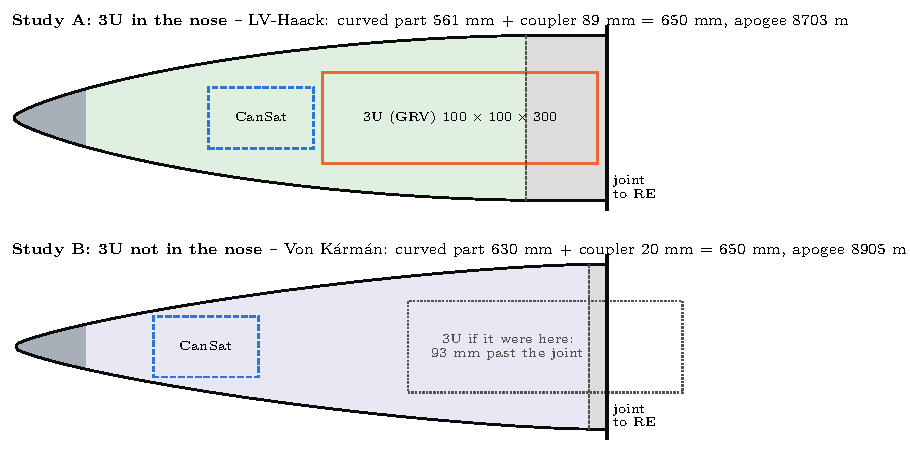
\includegraphics[width=\textwidth]{fig_tl_designs}
\caption{The two designs to scale (mm). Grey: tip and coupler cylinder; thick line: joint
to the RE bay; orange: 3U; blue dashed: CanSat; grey dotted (B): where the 3U would sit if it were in
the nose.}
\label{fig:designs}
\end{figure}

\begin{table}[H]
\centering
\caption{The two nose cones. Positions from the physical tip.}
\label{tab:final}
\small
\begin{tabular}{@{}>{\raggedright\arraybackslash}p{3.3cm}>{\raggedright\arraybackslash}p{6.0cm}>{\raggedright\arraybackslash}p{6.0cm}@{}}
\toprule
 & \textbf{A: 3U in the nose} & \textbf{B: 3U not in the nose} \\
\midrule
Profile & LV-Haack, Haack series $C = \tfrac13$ & Von K\'arm\'an, Haack series $C = 0$ \\
\multicolumn{3}{@{}l}{\quad Haack series: $y = \dfrac{R}{\sqrt\pi}\sqrt{\theta-\tfrac12\sin 2\theta + C\sin^3\theta}$,
$\theta=\arccos\!\left(1-\dfrac{2x}{L}\right)$, $x$ from the apex, $R = \SI{90}{mm}$} \\[4pt]
Curved length $L$ (to the theoretical apex) & \TLInLVHL{} ($L/D = \TLInLVHLD$); \TLInLVHPHYS{} physical & \TLOutVKL{} ($L/D = \TLOutVKLD$); \TLOutVKPHYS{} physical \\
Coupler cylinder & \TLInLVHC, full diameter, tangent & \TLOutVKC, full diameter, tangent \\
Total length & \SI{650}{mm} (\TLInLVHTOTPHYS{} physical) & \SI{650}{mm} (\TLOutVKTOTPHYS{} physical) \\
3U & front face at \TLInLVHXGRV; \TLInLVHLIN{} in the curved part, \TLInLVHINC{} in the cylinder & elsewhere in the vehicle \\
CanSat (needs \SI{115}{mm}) & \TLInLVHCAN{} of length with $r \geq \SI{39.2}{mm}$ ahead of the 3U & \TLOutVKCAN{} of length with $r \geq \SI{39.2}{mm}$ \\
Nose CP (Barrowman) & \TLInLVHXCP{} from the tip & \TLOutVKXCP{} from the tip \\
Apogee (model) & \TLInLVHAPO{} (\TLInLVHD); $M_{\max} = \TLInLVHMMAX$ & \TLOutVKAPO{} (\TLOutVKD); $M_{\max} = \TLOutVKMMAX$ \\
Static margin change & \TLInLVHDSM{} cal vs.\ the LVS nose & \TLOutVKDSM{} cal (nose only; without the 3U shift) \\
Both & \multicolumn{2}{p{12.2cm}}{\raggedright Tip: sphere $r_n = \SI{4.5}{mm}$. Diameter \SI{180}{mm}.} \\
Geometry files & {\footnotesize\TLInLVHFILE} & {\footnotesize\TLOutVKFILE} \\
\bottomrule
\end{tabular}
\end{table}

\subsection{CAD for the Fluent runs}

The six design points of Table~\ref{tab:designs} (three profiles, two studies) are exported as
solids of revolution in mm, $x$ from the physical tip, made of the blunted profile, the coupler
cylinder and a flat base at the joint: STEP (OpenCASCADE B-spline through 200 points), watertight
STL and the profile CSV. The STEP and CSV files are in \texttt{CFD/geometry\_650/} of the repository
(STL in \texttt{output/weisshorn\_650/total\_length/cad/}); the STEP volumes agree with the STL
within 0.1\,\%. They replace the \SI{810}{mm} geometry in the Fluent workflow note of the
\texttt{CFD} folder; the set-up, Mach numbers and meshing are unchanged.


\end{document}
